% Vector charts for the manuscript. Values supplied in the text are also
% used to position markers and shade cells when LaTeX rebuilds the paper.
\usepackage{tikz}
\usetikzlibrary{arrows.meta,positioning}
\usepackage{pgfplots}
\usepackage{pgfplotstable}
\usepgfplotslibrary{groupplots}
\pgfplotsset{compat=1.18}
\definecolor{evidenceBlue}{HTML}{28516F}
\definecolor{evidenceTeal}{HTML}{0C7468}
\definecolor{evidenceOchre}{HTML}{A54C20}
\definecolor{evidenceGray}{HTML}{65727B}
\newcommand{\scorepoint}[1]{%
  \begin{tikzpicture}[x=.024in,y=1ex,baseline=-.4ex]
    \draw[black!25] (0,0) -- (30,0);
    \foreach \x in {0,10,20,30}{\draw[black!25] (\x,-.22)--(\x,.22);}
    \fill[evidenceBlue] ({#1-55},0) circle[radius=1.8pt];
  \end{tikzpicture}}
\newcommand{\meanpoint}[2]{$#1 \pm #2$ & \scorepoint{#1}}
\newcommand{\bestmeanpoint}[2]{$\mathbf{#1 \pm #2}$ & \scorepoint{#1}}
\newcommand{\pointvalue}[1]{#1 & \scorepoint{#1}}
\newcommand{\gainbar}[1]{%
  \begin{tikzpicture}[x=.12in,y=1ex,baseline=-.4ex]
    \fill[black!10] (0,-.32) rectangle (6,.32);
    \fill[evidenceTeal] (0,-.32) rectangle (#1,.32);
  \end{tikzpicture}}
\newcommand{\scorepair}[2]{%
  \makebox[2.2em][r]{#1}\,\begin{tikzpicture}[x=.019in,y=1ex,baseline=-.4ex]
    \draw[black!18] (0,0)--(48,0);
    \draw[evidenceTeal,line width=1.15pt] ({#1-50},0)--({#2-50},0);
    \draw[evidenceBlue,fill=white] ({#1-50},0) circle[radius=1.75pt];
    \fill[evidenceTeal] ({#2-50},0) circle[radius=1.65pt];
  \end{tikzpicture}\,\makebox[2.2em][l]{#2}}
\newcommand{\acccell}[1]{%
  \pgfmathsetmacro{\cellweight}{max(0,min(66,(#1-50)*1.4))}%
  \edef\nextcell{\noexpand\cellcolor{evidenceTeal!\cellweight}}\nextcell\strut #1}
\newcommand{\losscell}[1]{%
  \pgfmathsetmacro{\cellweight}{min(65,#1*4)}%
  \edef\nextcell{\noexpand\cellcolor{evidenceOchre!\cellweight}}\nextcell\strut $-#1$}
\newcommand{\confidencecell}[1]{%
  \pgfmathsetmacro{\cellweight}{#1*64}%
  \edef\nextcell{\noexpand\cellcolor{evidenceBlue!\cellweight}}\nextcell\strut #1}
\newcommand{\modelmatch}[2]{%
  \begin{tikzpicture}[x=.0081in,y=1ex,baseline=-.4ex]
    \fill[black!11] (0,-.35) rectangle (137,.35);
    \fill[#2] (0,-.35) rectangle (#1,.35);
  \end{tikzpicture}\,#1}
\newcommand{\studyflow}{%
  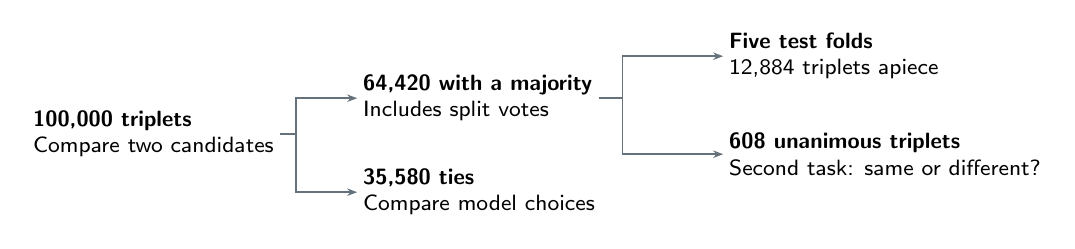
\begin{tikzpicture}[x=1in,y=1in,font=\sffamily\footnotesize,
    stage/.style={align=left,anchor=west,inner sep=2pt},
    arr/.style={-{Stealth[length=3.6pt]},draw=evidenceGray,line width=.55pt}]
    \node[stage] (a) at (0,0) {\textbf{100,000 triplets}\\Compare two candidates};
    \node[stage] (b) at (1.65,.18) {\textbf{64,420 with a majority}\\Includes split votes};
    \node[stage] (c) at (1.65,-.29) {\textbf{35,580 ties}\\Compare model choices};
    \node[stage] (d) at (3.48,.39) {\textbf{Five test folds}\\12,884 triplets apiece};
    \node[stage] (e) at (3.48,-.10) {\textbf{608 unanimous triplets}\\Second task: same or different?};
    \draw[arr] (a.east) -- ++(.08,0) |- (b.west);
    \draw[arr] (a.east) -- ++(.08,0) |- (c.west);
    \draw[arr] (b.east) -- ++(.12,0) |- (d.west);
    \draw[arr] (b.east) -- ++(.12,0) |- (e.west);
  \end{tikzpicture}}
% All four series use the same six measured epochs. No points are interpolated
% for unobserved epochs; straight connections only guide the eye.
\pgfplotstableread{
epoch clean change center surround
0 84.6 1.9 2.0 7.1
1 89.8 5.1 5.7 12.2
2 87.6 4.9 7.4 12.6
3 87.3 6.5 7.7 14.0
5 86.7 8.0 9.5 16.9
8 85.3 12.4 14.6 19.0
}\epochdata
\newcommand{\epochfigure}{%
  \begin{tikzpicture}
    \begin{groupplot}[group style={group size=2 by 1,horizontal sep=.48in},
      width=2.42in,height=1.36in,scale only axis=false,
      xmin=-.25,xmax=8.25,xtick={0,1,2,3,5,8},xlabel={Training epoch},
      tick label style={font=\sffamily\scriptsize},label style={font=\sffamily\footnotesize},
      title style={font=\sffamily\footnotesize\bfseries},axis lines=left,axis line style={black!45},
      tick style={black!45},ymajorgrids,grid style={black!12},/tikz/mark size=1.8pt,
      legend style={font=\sffamily\scriptsize,draw=none,fill=none,inner sep=1pt}]
    \nextgroupplot[title={Original images},ylabel={Accuracy (\%)},ymin=83,ymax=91,ytick={84,86,88,90}]
      \addplot[evidenceBlue,thick,mark=*] table[x=epoch,y=clean]{\epochdata};
    \nextgroupplot[title={Altered images},ylabel={Percentage points},ymin=0,ymax=20,ytick={0,5,10,15,20}]
      \addplot[evidenceTeal,thick,mark=*] table[x=epoch,y=change]{\epochdata};
      \addplot[evidenceBlue,thick,dashed,mark=square*] table[x=epoch,y=center]{\epochdata};
      \addplot[evidenceOchre,thick,dotted,mark=triangle*] table[x=epoch,y=surround]{\epochdata};
    \end{groupplot}
  \end{tikzpicture}}
